%% Journal manuscript, IEEE Transactions format
%% Compile:  tectonic report.tex
\documentclass[journal]{IEEEtran}

%% Times-metric fonts (IEEE house style); also ensures bold/italic actually load
%% under the XeTeX engine used by tectonic.
\usepackage{fontspec}
\setmainfont{Liberation Serif}
\setsansfont{Liberation Sans}
\setmonofont{Liberation Mono}

\usepackage{graphicx}
\usepackage{amsmath}
\usepackage{amssymb}
\usepackage{booktabs}
\usepackage{url}
\usepackage[hidelinks]{hyperref}

\begin{document}

\title{Beyond Recall: Metre-Level Evaluation and\\
Grid-Free Decoding for UAV Self-Positioning}

\author{Anonymous Author(s)%
\thanks{Manuscript prepared \today. Code and evaluation scripts build on the public
DenseUAV repository; all added scripts are separate files and leave the original
evaluation code unmodified.}}

\markboth{Manuscript draft --- not yet submitted}%
{Beyond Recall: Metre-Level Evaluation and Grid-Free Decoding for UAV Self-Positioning}

\maketitle

\begin{abstract}
GPS-denied unmanned aerial vehicles (UAVs) must localise themselves visually, and the
dominant paradigm formulates this as retrieval against a geo-tagged satellite gallery.
On the DenseUAV benchmark, successive methods have pushed Recall@1 from roughly 81\% to
89\%, and this number is treated as the field's measure of progress. We show that such
gains are bounded by a \emph{quantisation ceiling}: because the system can only return
the centre coordinate of a discrete gallery cell, the localisation error cannot fall
below a fixed geometric bound. Measuring the gallery directly, we find a sampling step
of $s \approx 19.71$\,m, implying a median error floor of $\approx 7.86$\,m regardless
of retrieval quality. Training four architectures under an identical decoding rule
(Recall@1 spanning 33\%--83\%), we find a more severe problem: DenseUAV publishes no
continuous ground-truth position for UAV images, so the metre-based metrics reported in
this line of work (SDM, MA@$K$) collapse into a near-monotone transform of Recall@1 and
are flat over the entire $1$--$17$\,m range. These metrics also hide tail risk: one
architecture trails the baseline by 1.46 Recall@1 points yet has a $6.3\times$ larger
95th-percentile error (1193\,m vs.\ 189\,m). We propose a metre-level protocol
(median/p90/p95 and the full error CDF) and evaluate a training-free weighted-centroid
decoder. An exhaustive sweep of its two hyper-parameters shows that \emph{no} setting
beats plain top-1 decoding, because feature-space neighbours are not geographic
neighbours. We analyse why, and derive the design constraints that a corrected decoder
must satisfy.
\end{abstract}

\begin{IEEEkeywords}
UAV self-positioning, cross-view geo-localisation, GPS-denied navigation, evaluation
metrics, benchmark validity, image retrieval.
\end{IEEEkeywords}

\section{Introduction}
UAVs operating in low-altitude urban environments frequently lose GPS
service through multipath interference, occlusion, or deliberate spoofing, and must then
fall back on vision to determine their own position. The prevailing approach casts this
as \emph{cross-view geo-localisation}: an image captured by the UAV is matched against a
gallery of geo-tagged satellite tiles, and the UAV position is inferred from the
best-matching tile.

On the DenseUAV benchmark~\cite{denseuav}, a sequence of methods --- FSRA~\cite{fsra},
MCCG, and CEUSP~\cite{ceusp} --- has raised Recall@1 (R@1) from about 81\% to 89\%.
This single number has become the field's proxy for progress.

This paper asks a question that the R@1-driven literature leaves unanswered:
\emph{how many metres of localisation accuracy does a several-point gain in R@1 actually
buy?} Our answer, established both analytically and empirically, is: \textbf{very close
to none}, for two compounding reasons.

First, a retrieval system can only emit the coordinate of a discrete gallery element.
The error is therefore lower-bounded by the gallery sampling step $s$, no matter how
accurate the retrieval stage becomes (Section~\ref{sec:ceiling}).

Second --- and more seriously --- the public ground truth of DenseUAV is \emph{itself}
quantised to the tile level. No continuous GPS coordinate is released for any individual
UAV image. Consequently the metre-based metrics introduced precisely to remedy the
shortcomings of R@1 are, on this benchmark, a near-monotone transform of R@1 and carry
almost no independent spatial information (Section~\ref{sec:metric}).

\textbf{Contributions.}
\begin{itemize}
\item An analysis of the quantisation ceiling of retrieval-based decoding, validated
against the sampling step measured directly from the released GPS data.
\item Evidence that SDM and MA@$K$ on DenseUAV degenerate into a step function of R@1,
uniformly across architectures spanning R@1 from 33\% to 83\% --- a limitation of
\emph{benchmark validity} rather than of any particular method.
\item A metre-level evaluation protocol (median, p90, p95, full CDF) applied to four
retrained architectures, showing that p95 separates tail risk that neither R@1 nor SDM
reveals.
\item A training-free weighted-centroid decoder together with an exhaustive
hyper-parameter sweep, an honest negative result, and the resulting design constraints
for a corrected decoder.
\end{itemize}

\begin{figure}[!t]
\centering
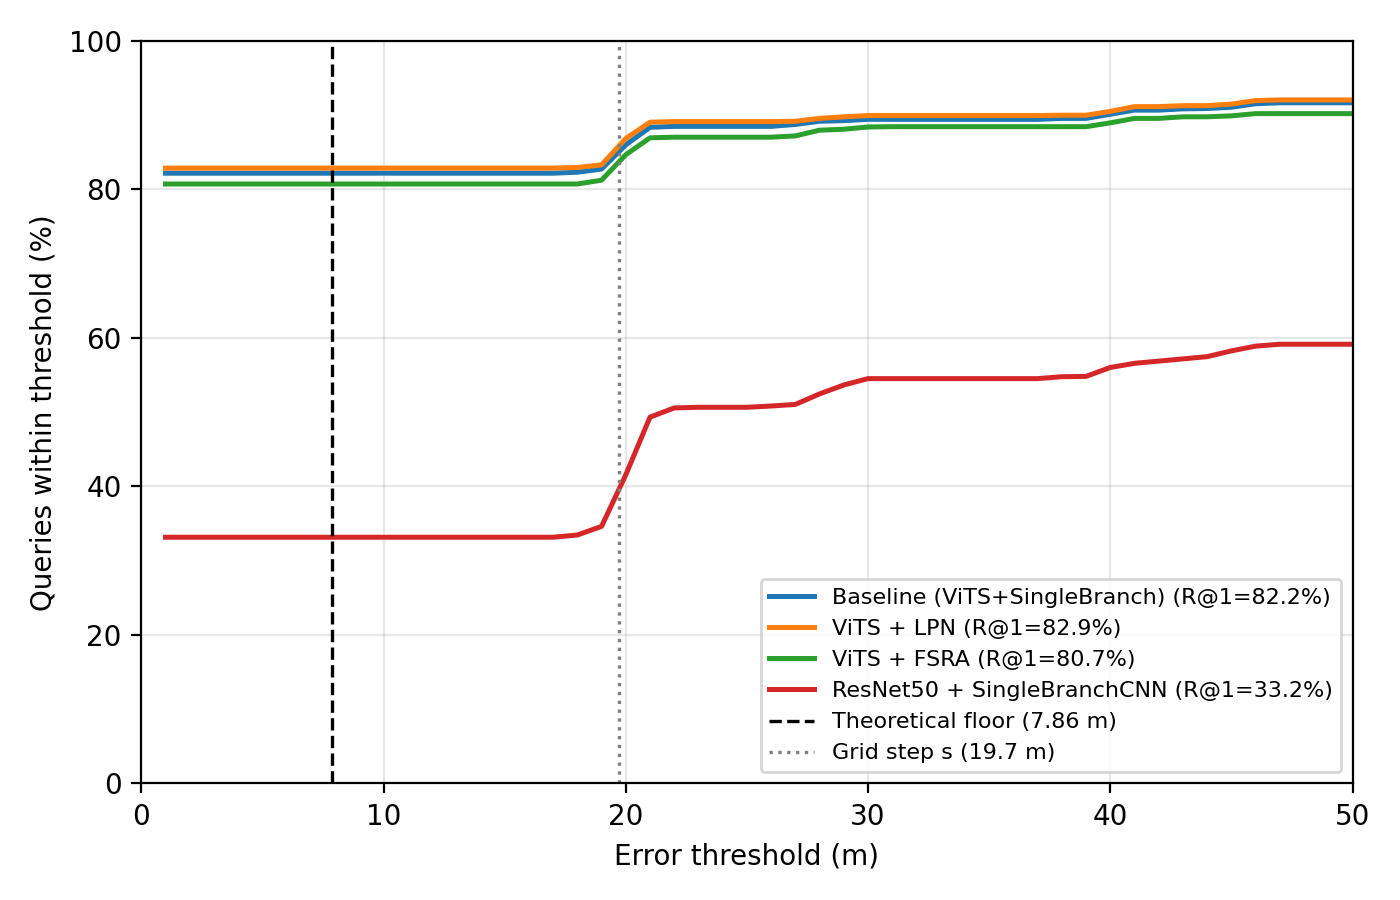
\includegraphics[width=\columnwidth]{docs/images/fig1_cdf.png}
\caption{Error CDF for four architectures sharing an identical decoding rule
(top-1 $\rightarrow$ gallery cell centre). All four curves are exactly flat until the
measured sampling step $s \approx 19.7$\,m and only then jump, including ResNet50 whose
R@1 is merely 33\%. The theoretical floor of 7.86\,m lies inside the flat region of
every curve and is entirely inert with respect to the 33\%--83\% spread in R@1.}
\label{fig:cdf}
\end{figure}

\section{Related Work}

\textbf{Cross-view geo-localisation.} The field began with ground-to-aerial matching and
later moved to drone-to-satellite settings through University-1652, SUES-200, and
DenseUAV~\cite{denseuav}; we use the last of these, which targets dense urban scenes.

\textbf{Methods on DenseUAV.} FSRA~\cite{fsra}, MCCG, CEUSP~\cite{ceusp} and DINOv2-based
variants all optimise retrieval metrics (R@1, SDM@$K$) and treat them as the terminal
objective.

\textbf{Precise positioning rather than correct retrieval.} VIGOR first abandoned the
centre-aligned assumption between UAV and satellite crops. FPI and OS-FPI recast the task
as regression of a continuous position inside a large satellite image. Notably, the
DenseUAV repository itself ships \texttt{evaluate\_RDS.py}, written for the FPI label
format, and the same group later released the DRL paradigm --- evidence that the original
authors also recognised the limitation we quantify here. More recently, a benchmark built
on local feature matching (RoMa, DKM, LoFTR) with re-ranking~\cite{camp2025} attains
metre-level accuracy on aerial and satellite reference maps (up to 74\% within 5\,m).

\textbf{Positioning of this work.} Those directions either require retraining under a
regression paradigm (FPI, DRL) or rebuild the entire pipeline around feature matching.
We instead study a \emph{training-free} post-processing step applicable to any existing
retrieval checkpoint --- and report why, on a benchmark with tile-quantised ground truth,
this turns out to be substantially harder than expected.

\section{The Quantisation Ceiling}
\label{sec:ceiling}

\subsection{Problem Formulation}
Retrieval decoding maps a UAV image to a discrete gallery element,
\begin{equation}
\hat{p} \;=\; g\!\left(\arg\max_{i}\ \mathrm{sim}\!\left(f_{q},\, f_{g,i}\right)\right),
\end{equation}
where $g(i)$ is the pre-assigned centre coordinate of gallery cell $i$. Since $g$ takes
values in a finite set, the error $\lVert \hat{p}-p_{\text{true}} \rVert$ can never be
smaller than the distance from $p_{\text{true}}$ to the nearest cell centre, however
accurate the retrieval stage.

\subsection{Lower Bound}
For a gallery sampled on a uniform grid of step $s$, the Voronoi cell of each gallery
point is an $s \times s$ square. If the query position is uniform within that cell, the
distance $r$ to the cell centre satisfies $P(r \le x) = \pi x^{2}/s^{2}$ for
$x \le s/2$, so the median is
\begin{equation}
x_{50} \;=\; \sqrt{\tfrac{0.5}{\pi}}\; s \;\approx\; 0.399\,s .
\label{eq:floor}
\end{equation}
Table~\ref{tab:floor} instantiates \eqref{eq:floor} for typical sampling steps.

\begin{table}[!t]
\centering
\caption{Theoretical median error floor as a function of sampling step $s$.}
\label{tab:floor}
\begin{tabular}{lccc}
\toprule
$s$ (m) & 10 & 20 & 40 \\
\midrule
Median floor $\approx 0.399s$ (m) & 3.99 & 7.98 & 15.96 \\
\bottomrule
\end{tabular}
\end{table}

\subsection{Measured Sampling Step of DenseUAV}
We computed the haversine distance from every test-set gallery tile ($N=3033$) to its
nearest neighbour, using the coordinates in \texttt{Dense\_GPS\_ALL.txt}:

\begin{center}
\begin{tabular}{ccccc}
\toprule
min & p10 & \textbf{median} & p90 & max \\
\midrule
9.41 & 18.62 & \textbf{19.71} & 19.99 & 20.88 \\
\bottomrule
\end{tabular}
\end{center}

The distribution is tightly concentrated near 20\,m, so the gallery is effectively a
uniform grid with $s \approx 19.71$\,m, giving a median floor of
$x_{50} \approx 0.399 \times 19.71 \approx \mathbf{7.86}$\,m.

\section{Metre-Level Evaluation}
\label{sec:metric}

\subsection{Why the Published Metre-Based Metrics Do Not Fix R@1}
The standard argument --- made in DenseUAV itself --- is that binary R@1 ignores spatial
error, motivating metre-based metrics such as SDM and MA@$K$. Our experiments show this
holds in principle but \emph{fails on DenseUAV itself}, for a structural reason:
\texttt{Dense\_GPS\_ALL.txt}, the only ground-truth source, contains coordinates for
satellite tiles keyed by class identifier, and \emph{no} continuous GPS for drone images.
We verified that the drone JPEGs carry no EXIF GPS and that no other metadata file exists.
When the evaluation code looks up the "true" position of a drone query, it therefore
resolves the query's own class identifier and returns the centre of the paired satellite
tile.

The measured consequence, identical across all four trained architectures
(Table~\ref{tab:main}, Fig.~\ref{fig:cdf}), is
\begin{equation}
\text{MA@1m} = \text{MA@2m} = \cdots = \text{MA@17m} \approx \text{R@1},
\end{equation}
followed by a jump exactly at $s \approx 20$\,m. In other words: a correct class implies
$\approx 0$\,m error (the same coordinate is retrieved twice), while an incorrect class
implies an error of at least one grid step. Nothing lies in between. On this benchmark
SDM and MA@$K$ are thus essentially a monotone re-expression of R@1. Crucially, this
holds across the \emph{entire} R@1 range we tested (33\%--83\%), which rules out the
possibility that the step behaviour is an artefact of strong models only; it is a
structural property of the labels, independent of backbone quality.

\subsection{What R@1 and SDM Conceal: Tail Risk}
Per-query medians are $0.00$\,m for the three architectures with $\text{R@1}>50\%$ --- a
direct consequence of the quantised ground truth, since once more than half the queries
are correct the median falls inside the zero-error branch. For ResNet50
($\text{R@1}=33.16\%<50\%$) the median jumps to 21.41\,m, not because the model degrades
smoothly in metres but because most queries fall on the "wrong class" branch of the same
step function. This is further evidence that median and MA@$K$ on this benchmark mainly
report retrieval correctness rather than continuous positioning error.

The p90 and p95 statistics, by contrast, differ sharply even between architectures with
near-identical R@1. FSRA trails the baseline by 1.46 R@1 points yet exhibits a
$6.3\times$ larger p95 (1193\,m vs.\ 189\,m): its worst 5\% of queries are occasionally
matched to an entirely different campus among the 14 universities in the dataset. This is
a safety-critical failure mode that neither R@1 nor SDM exposes.

Independent corroboration appears in the published literature: in the CEUSP results
table~\cite{ceusp}, the DenseUAV baseline attains a \emph{higher} SDM@1 (86.50) than MCCG
(85.94) despite a lower R@1 (83.01 vs.\ 83.14) --- a genuine rank inversion between the
two metrics, requiring no simulation.

\subsection{Proposed Protocol}
We recommend reporting the median, p90, p95, the fraction within fixed radii
($<5$\,m, $<10$\,m), and the full error CDF, with p95 given priority because it is the
quantity that governs flight safety.

\section{Grid-Free Decoding}
\label{sec:decoder}

\subsection{Weighted Centroid}
Instead of returning the top-1 coordinate alone, we form the similarity-weighted centroid
of the top-$K$ candidates,
\begin{equation}
\hat p \;=\; \frac{\sum_{i=1}^{K} w_i\, g(i)}{\sum_{i=1}^{K} w_i},
\qquad
w_i \;=\; \exp\!\left(\frac{s_i - \max_j s_j}{\tau}\right),
\label{eq:centroid}
\end{equation}
where $s_i$ is the cosine similarity of candidate $i$. This is pure post-processing on
already-extracted features and requires \textbf{no retraining}.

\subsection{Negative Result and Its Cause}
Table~\ref{tab:ablation} reports an exhaustive sweep of $(K,\tau)$ on the baseline
checkpoint. The error increases monotonically in both parameters; the best configuration
is the limit $\tau \to 0$, $K = 1$ --- that is, plain top-1 decoding with no blending at
all. No sweet spot exists anywhere in the searched space, so the failure is not a matter
of insufficient tuning. Two causes compound:

\begin{enumerate}
\item When top-1 is already correct (80--83\% of queries), the error is already
$\approx 0$\,m by construction of the labels (Section~\ref{sec:metric}); blending any
other candidate can only move the estimate away from an exactly correct value. There is
nothing to smooth.
\item Top-$K$ neighbours in feature space are \emph{not} guaranteed to be geographic
neighbours. The second- or third-ranked candidate may belong to a different campus
hundreds or thousands of metres away, dragging the centroid far off.
\end{enumerate}

A revealing exception occurs on ResNet50 ($\text{R@1}=33.16\%$, most queries incorrect):
the median still degrades with $K$ ($21.41 \rightarrow 339.61$\,m) but p95 \emph{improves}
slightly ($3807 \rightarrow 2862$\,m). When top-1 is frequently wrong and close to random,
averaging does suppress extreme outliers --- the opposite of the high-R@1 regime. The
benefit of centroid decoding is therefore regime-dependent, which a fixed $K$ cannot
accommodate and a confidence gate must handle explicitly.

\section{Experiments}

\subsection{Setup}
\textbf{Data.} DenseUAV as released: 6{,}768 UAV and 13{,}536 satellite training images
over 2{,}256 classes from 10 universities; 777 query-drone classes and 3{,}033
gallery-satellite classes from 4 non-overlapping universities for testing, with three
flight altitudes (H80/H90/H100) per class.

\textbf{Hardware and hyper-parameters.} A single RTX 3060 (12\,GB). We retain the original
\texttt{train\_test\_local.sh} settings: $\mathrm{lr}=0.01$, batch size 16, one class
block, 512-dimensional bottleneck, $224 \times 224$ inputs, 120 epochs, and the
CELoss + WeightedSoftTripletLoss + KLLoss objective. Throughput is 15--19\,s per epoch,
i.e.\ 30--40 minutes per configuration.

\textbf{Controlled variable.} The only quantity varied across the four configurations is
the architecture (backbone/head); the decoding rule is held fixed at
top-1~$\rightarrow$~cell centre. Every difference in Fig.~\ref{fig:cdf} is therefore
attributable to the architecture, and every \emph{similarity} --- notably the location of
the jump --- to the decoding rule.

\subsection{Reproducibility}
Our retrained baseline reaches $\text{R@1}=82.20\%$ against the 83.01\% published for the
equivalent configuration, i.e.\ \textbf{99.0\%} of the original result (a gap of 0.81
points), consistent with differences in seed, library version (PyTorch 2.0 vs.\ 1.10) and
hardware. We consider the pipeline faithfully reproduced.

\subsection{Main Results}
Table~\ref{tab:main} and Fig.~\ref{fig:cdf} summarise the outcome. Three observations
follow.

\begin{table*}[!t]
\centering
\caption{Main results on the DenseUAV test set. Median/p90/p95 are computed per query as
the haversine distance to the retrieved top-1 tile centre. All four configurations share
an identical decoding rule.}
\label{tab:main}
\begin{tabular}{lcccccc}
\toprule
Method & R@1 (\%) & R@5 (\%) & SDM@1 & Median (m) & p90 (m) & p95 (m) \\
\midrule
ViTS + SingleBranch (baseline) & 82.20 & 94.77 & 85.26 & 0.00 & 39.87 & 188.55 \\
ViTS + LPN                     & 82.88 & 95.02 & 85.80 & 0.00 & 37.36 & 159.66 \\
ViTS + FSRA                    & 80.74 & 93.78 & 83.80 & 0.00 & 45.28 & \textbf{1193.27} \\
ResNet50 + SingleBranchCNN     & 33.16 & 57.36 & 41.63 & 21.41 & \textbf{2679.08} & \textbf{3807.46} \\
\bottomrule
\end{tabular}
\end{table*}

\begin{enumerate}
\item \textbf{The jump location is invariant.} Although R@1 ranges from 33.16\% to
82.88\%, every CDF is exactly flat up to $\approx17$--$19$\,m and jumps at
$s \approx 19.7$\,m. The \emph{height} of the plateau tracks R@1; its \emph{position}
does not.
\item \textbf{SDM tracks R@1.} Across all four configurations the SDM@1 ranking matches
the R@1 ranking exactly, and the gap between the two is nearly constant
($\approx 3.0$--$3.1$ points within the ViT group). SDM supplies no independent ranking
information here.
\item \textbf{p95 is decoupled.} FSRA and the baseline differ by 1.46 R@1 points but by a
factor of 6.3 in p95. Neither R@1 nor SDM predicts p95.
\end{enumerate}

\subsection{Decoder Hyper-Parameter Sweep}

\begin{table}[!t]
\centering
\caption{Sweep of $\tau$ and $K$ for the weighted-centroid decoder of
\eqref{eq:centroid} on the baseline checkpoint. All values in metres; lower is better.}
\label{tab:ablation}
\begin{tabular}{lcccccc}
\toprule
& \multicolumn{2}{c}{$K=3$} & \multicolumn{2}{c}{$K=5$} & \multicolumn{2}{c}{$K=10$} \\
\cmidrule(lr){2-3}\cmidrule(lr){4-5}\cmidrule(lr){6-7}
$\tau$ & p90 & p95 & p90 & p95 & p90 & p95 \\
\midrule
0.01 & 65.84  & 818.75  & 87.66  & 852.25  & 98.44   & 862.69 \\
0.02 & 99.57  & 990.25  & 210.96 & 991.31  & 279.85  & 1020.95 \\
0.05 & 141.47 & 1088.94 & 502.08 & 1062.47 & 688.11  & 1197.18 \\
0.10 & 139.45 & 1114.99 & 634.82 & 1162.35 & 931.03  & 1398.40 \\
0.50 & 144.59 & 1169.81 & 810.05 & 1379.64 & 1176.49 & 1660.25 \\
\midrule
\multicolumn{7}{l}{\emph{Reference --- plain top-1 ($K=1$): p90 $=39.87$, p95 $=188.55$}}\\
\bottomrule
\end{tabular}
\end{table}

The sweep is monotone in both directions, and every entry is worse than the top-1
reference row. This establishes the negative result exhaustively rather than at a single
lucky operating point: the flawed assumption is that feature-space proximity implies
geographic proximity, not that the parameters were poorly chosen.

\subsection{Failure Analysis}
\textbf{Cross-site confusion.} p95 values in the hundreds to thousands of metres show that
failing queries are not confused with adjacent cells but with entirely different areas ---
plausible given that the test split spans four universities with visually similar urban
fabric (rooftops, courtyards, service roads). This is both the most dangerous failure mode
for real flight and the direct cause of the centroid decoder's failure.

\textbf{Architecture-family sensitivity.} ResNet50 reaches only 33.16\% R@1 under
hyper-parameters tuned for ViT ($\mathrm{lr}=0.01$). We deliberately did not retune, since
the objective is to probe the \emph{decoding ceiling} rather than to maximise performance,
and a weak model is a useful probe of the step behaviour in the low-R@1 regime.

\textbf{Homogeneous regions and temporal change.} The dataset provides both current and
historical (\texttt{\_old}) satellite imagery for each site; texture-homogeneous areas
(car parks, sports fields, large flat roofs) are the principal source of confusion. We did
not isolate this factor quantitatively, which would require manual terrain-type labels.

\section{Discussion and Limitations}
The quantisation ceiling is a design choice, not a physical limit: satellite imagery at the
zoom level used by DenseUAV resolves well below one metre per pixel, so the information
required to localise far more precisely than 7--8\,m is present in the imagery and simply
discarded by the discrete-retrieval paradigm.

The benchmark limitation is our principal finding rather than an aside. Because DenseUAV
--- and plausibly related drone-to-satellite datasets --- publishes no continuous UAV
position, no claim of metre-level precision on this benchmark can be validated
independently of whether retrieval selected the correct class.

Limitations of this study: (i) we have not yet implemented the spatially gated decoder,
only established that it is required; (ii) we have no experiments on a benchmark with
genuinely continuous ground truth, which is needed to validate
Section~\ref{sec:decoder} independently; (iii) the four configurations vary only in
backbone and head, at a single input resolution.

\section{Directions for Improvement}
Ordered by priority according to the evidence in this study.

\subsection{Spatial Confidence Gating}
Table~\ref{tab:ablation} isolates the core problem: top-$K$ feature neighbours need not be
geographic neighbours. The direct remedy is to filter candidates \emph{before} blending:
anchor on $g(1)$; discard any candidate with $\lVert g(i)-g(1)\rVert > \rho$ for $\rho$ a
small multiple of the grid step (e.g.\ $\rho = 3s \approx 60$\,m); blend the remainder, and
fall back to plain top-1 if none survive. This preserves the "never worse than top-1"
property that \eqref{eq:centroid} currently violates. A complementary confidence gate can
use the top-1/top-2 score margin: when the model is decisive, return top-1 directly and
blend only when it hesitates among geographically close candidates. The cost is negligible
and no retraining is needed.

\subsection{Migrating to a Benchmark with Continuous Ground Truth}
No sub-tile decoding improvement is verifiable on DenseUAV. FPI and OS-FPI provide
continuous UAV positions inside large satellite images, and the DenseUAV repository already
contains \texttt{evaluate\_RDS.py} written for that label format, so integration cost is
low. Only there can the question "how many metres does continuous decoding actually save?"
be answered.

\subsection{Geometric Refinement by Feature Matching}
Once the correct tile is selected, a similarity transform between the UAV image and that
tile can be estimated with local feature matching (LoFTR, RoMa, DKM) and the precise
in-tile position recovered --- shown feasible by~\cite{camp2025} (up to 74\% within 5\,m).
Among the directions surveyed this is the only one capable of breaking the 7.86\,m ceiling
outright, since it exploits the sub-metre pixel resolution of the satellite imagery. The
risk is a low matching success rate in homogeneous areas, again requiring a confidence gate
that falls back to top-1.

\subsection{Improving the Dataset and Protocol}
Releasing the continuous UAV coordinates --- already present in the flight logs used during
collection --- would be the cheapest change with the largest effect, making true positioning
error measurable for the whole research line. Adding queries captured \emph{between} grid
cells would test the realistic case in which the UAV does not overfly a sampling point.
Finally, we suggest that future work on this benchmark report p90/p95 in metres alongside
R@1 and SDM, since in our study p95 was the only statistic that revealed tail risk.

\subsection{Broader Sweeps}
The present configurations share a single $224 \times 224$ input resolution. Natural
extensions are higher resolutions (384, 512), a per-altitude breakdown using the existing
H80/H90/H100 labels, and CNN-specific hyper-parameter tuning for a fairer ResNet50
comparison.

\section{Conclusion}
We have shown that Recall@1 gains on the DenseUAV benchmark do not translate into
metre-level accuracy, for a reason more fundamental than the retrieval quality of any
given method. The gallery imposes a geometric floor of $\approx 7.86$\,m at the measured
sampling step of 19.71\,m, and the released ground truth is itself quantised to that same
grid, so the metre-based metrics used in this literature reduce to a step function of
Recall@1 across the full 33\%--83\% range we tested. Tail risk, which these metrics hide
entirely, varies by a factor of 6.3 between architectures separated by 1.46 Recall@1
points. A training-free weighted-centroid decoder does not resolve this: an exhaustive
hyper-parameter sweep shows that plain top-1 decoding is optimal, because feature-space
neighbours are not geographic neighbours. Progress on precise UAV self-positioning
therefore requires spatially gated decoding, geometric refinement that exploits sub-metre
imagery, and --- most importantly --- benchmarks whose ground truth is not quantised to the
retrieval grid.

\appendices
\section{Implementation Details}
The conda environment provides Python 3.10 and PyTorch 2.0.0+cu118. An initial
\texttt{RuntimeError: Numpy is not available} arose from an ABI conflict between
\texttt{numpy 2.2.6} and \texttt{torch 2.0.0}; installing \texttt{numpy<2} resolves it
(\texttt{opencv-python} declares \texttt{numpy>=2} but operates correctly with 1.26.4).

Pairing a CNN backbone with a transformer head raises
\texttt{mat1 and mat2 shapes cannot be multiplied (112x7 and 2048x512)}, because
\texttt{SingleBranch} slices token sequences via \texttt{features[:,0]} whereas
\texttt{resnet50.forward\_features()} returns a $(B,C,H,W)$ feature map. The repository's
\texttt{SingleBranchCNN} head (adaptive average pooling) is the correct counterpart; no
modification of the original code is required. We also pass \texttt{--h 224 --w 224}
explicitly to \texttt{test.py}, whose default is $256 \times 256$ and would otherwise
mismatch the training resolution.

Added scripts: \texttt{run\_experiments.sh} (sequential train/evaluate over
configurations), \texttt{plot\_fig1\_cdf.py} (Fig.~\ref{fig:cdf} from the per-checkpoint
MA@$K$ output), and \texttt{eval\_weighted\_centroid.py} (post-processing of the stored
features for Section~\ref{sec:decoder}). The original evaluation code is left unmodified
so that results remain comparable with the published numbers.

\begin{thebibliography}{9}
\bibitem{denseuav}
M.~Dai, E.~Zheng, Z.~Feng, L.~Qi, J.~Zhuang, and W.~Yang,
``Vision-based UAV self-positioning in low-altitude urban environments,''
\emph{IEEE Trans. Image Process.}, vol.~33, pp.~493--508, 2024.

\bibitem{fsra}
M.~Dai \emph{et al.}, ``A transformer-based feature segmentation and region alignment
method for UAV-view geo-localization,'' \emph{IEEE Trans. Circuits Syst. Video Technol.},
2022.

\bibitem{ceusp}
``Precise GPS-denied UAV self-positioning via context-enhanced cross-view
geo-localization,'' arXiv:2502.11408, 2025.

\bibitem{camp2025}
``Exploring the best way for UAV visual localization under low-altitude multi-view
observation condition: a benchmark,'' arXiv:2503.10692, 2025.
\end{thebibliography}

\end{document}
